\section{Технологическая часть}
\subsection{Выбор средств реализации ПО}

\hspace{1.25cm}
Для разработки программы выбран язык программирования Python. Данный выбор обусловлен следующими причинами:

\begin{enumerate}
    \item \underline{Богатая экосистема инструментов и библиотек}\\ 
    Python поддерживает необходимые для проекта библиотеки, такие как:
    \begin{itemize}
        \item \textbf{Tkinter} для создания графического пользовательского интерфейса (GUI).
        \item \textbf{NumPy} для выполнения математических операций, включая преобразования координат и вычисления.
        \item \textbf{math} для работы с математическими функциями.
        \item \textbf{ProcessPoolExecutor} из модуля \textbf{concurrent.futures} для организации мультипроцессинга.
        \item \textbf{pytest} для написания модульных тестов, что помогает автоматизировать проверку функционала программы и выявлять ошибки.
    \end{itemize}

    \item \underline{Использование наработок из курса <<Компьютерная графика>>}\\ 
    Python и Tkinter уже применялись в лабораторных работах по курсу <<Компьютерная графика>>, где была отработана инфраструктура для создания приложений. Это позволило заимствовать проверенные решения, такие как:
    \begin{itemize}
        \item Интерфейсные элементы и их взаимодействие.
        \item Фрагменты кода для работы с объектами сцены.
        \item Систему тестирования и сборки, что ускорило разработку и снизило риск ошибок.
    \end{itemize}
    
    \item \underline{Поддержка объектно-ориентированного программирования (ООП)}\\ 
    Python предоставляет удобные механизмы для работы с ООП, что позволило разделить программу на независимые модули и классы (например, объекты сцены, камера, управление интерфейсом).

    \item \underline{Платформенная независимость}\\ 
    Программы на Python работают на различных операционных системах (Windows, macOS, Linux), что делает приложение доступным для широкого круга пользователей.

    \item \underline{Простота и читаемость кода}\\
    Python отличается лаконичным синтаксисом и высокой читаемостью кода, что ускоряет процесс разработки и тестирования программы. Это особенно важно для курсового проекта, где требуется не только реализовать функционал, но и ясно представить код и структуру программы.
\end{enumerate}



\subsection{Структура программы}

\hspace{1.25cm}
Программа представляет собой объектно-ориентированную архитектуру, предназначенную для работы с элементами сцены и пространственными объектами, такими как стены, двери и окна. Взаимодействие между классами организовано вокруг обработки и отображения трёхмерной модели помещения. Структура классов разработанного программного обеспечения представлена на рисунке~\ref{fig:class_UML}.

\begin{figure}[h!]
    \centering
    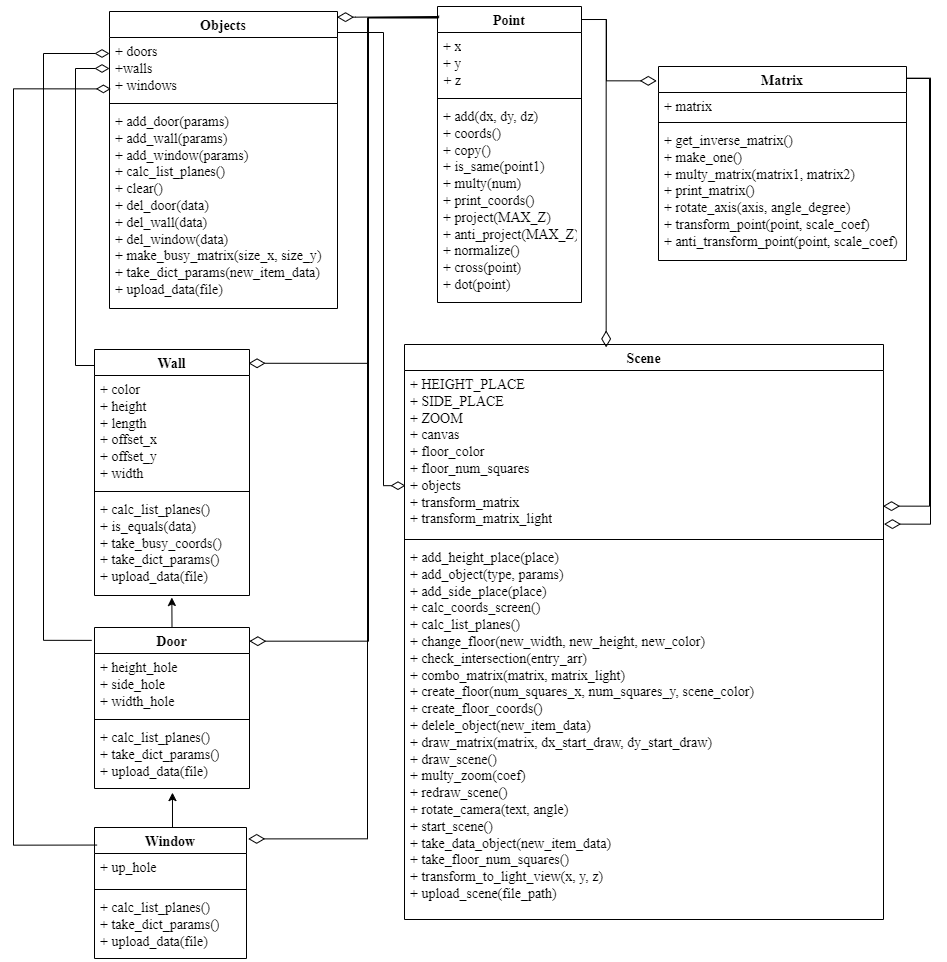
\includegraphics[width=1\textwidth]{img/class_UML.png}
    \caption{Структура классов разработанного программного обеспечения.}
    \label{fig:class_UML}
\end{figure}

\subsubsection{Классы и их роли}

\hspace{1.25cm}
Основные классы и их функции можно разбить на несколько ключевых компонентов.

\paragraph{Пространственные элементы}
\hspace{1.25cm}
Эти классы представляют объекты сцены (стены, двери, окна) и содержат свойства, необходимые для их описания, а также методы для вычисления их геометрии.
\begin{itemize}
    \item \textbf{Wall}:
    \begin{itemize}
        \item Хранит такие параметры, как цвет, длина, высота, ширина и смещение.
        \item Методы:
        \begin{itemize}
            \item \verb|calc_list_planes()|: вычисляет геометрические плоскости объекта.
            \item \verb|is_equals(data)|: проверяет эквивалентность с другим объектом.
            \item \verb|upload_data(file)|: загружает параметры объекта из файла.
        \end{itemize}
    \end{itemize}
    \item \textbf{Door} (наследует \textit{Wall}):
    \begin{itemize}
        \item Добавляет дополнительные свойства, такие как высота, ширина и сторона, где расположено отверстие.
    \end{itemize}
    \item \textbf{Window} (наследует \textit{Wall}):
    \begin{itemize}
        \item Включает параметр \verb|up_hole|, связанный с высотой окна.
    \end{itemize}
\end{itemize}

\paragraph{Работа с геометрическими преобразованиями}
\begin{itemize}
    \item \textbf{Matrix}:
    \begin{itemize}
        \item Хранит матрицы преобразований и предоставляет инструменты для выполнения операций с ними.
        \item Методы:
        \begin{itemize}
            \item \verb|get_inverse_matrix()|: получение обратной матрицы.
            \item \verb|mult_matrix()|: умножение двух матриц.
            \item \verb|rotate_axis()|: поворот объектов вокруг оси.
            \item \verb|transform_point()|: трансформация координат точки.
        \end{itemize}
    \end{itemize}
    \item \textbf{Point}:
    \begin{itemize}
        \item Представляет точку в пространстве с координатами $(x, y, z)$.
        \item Методы:
        \begin{itemize}
            \item \verb|add(dx, dy, dz)|: добавляет смещение к точке.
            \item \verb|multiply(num)|: умножает координаты на заданное число.
            \item \verb|project(MAX_Z)|: выполняет проекцию точки на плоскость.
        \end{itemize}
    \end{itemize}
\end{itemize}

\paragraph{Управление коллекцией объектов}
\textbf{Objects}:
\begin{itemize}
    \item Хранит списки объектов сцены (двери, стены, окна).
    \item Методы:
    \begin{itemize}
        \item \verb|add_door(params)|, \verb|add_wall(params)|, \verb|add_window(params)|: добавление объектов.
        \item \verb|calc_list_planes()|: вычисление плоскостей для всех объектов.
        \item \verb|clear()|: очистка списка объектов.
        \item \verb|check_intersection(entry_arr)|: проверка пересечений между объектами.
    \end{itemize}
\end{itemize}

\paragraph{Управление сценой}
\textbf{Scene}:
\begin{itemize}
    \item Основной класс для управления сценой и её параметрами.
    \item Свойства:
    \begin{itemize}
        \item Константы, такие как размеры сцены (\verb|HEIGHT_PLACE|, \verb|SIDE_PLACE|).
        \item Цвет пола, параметры света, матрица трансформации и объекты сцены.
    \end{itemize}
    \item Методы:
    \begin{itemize}
        \item \verb|add_object(type, params)|: добавление нового объекта в сцену.
        \item \verb|rotate_camera(text, angle)|: вращение камеры.
        \item \verb|draw_scene()|: отрисовка сцены.
        \item \verb|check_intersection(entry_arr)|: проверка пересечений объектов сцены.
    \end{itemize}
\end{itemize}

\subsubsection{Логика работы программы}
\begin{enumerate}
    \item \textbf{Инициализация сцены}\\
    Создаётся объект \textit{Scene}, в который добавляются стены, двери и окна через методы \verb|add_object| или \verb|add_wall|.
    \item \textbf{Работа с геометрией}\\
    Методы классов \textit{Wall}, \textit{Door} и \textit{Window} используются для вычисления параметров объектов, а класс \textit{Matrix} помогает выполнять геометрические преобразования.
    \item \textbf{Проверка пересечений}\\
    Программа может проверять пересечения между объектами сцены с помощью метода \verb|check_intersection|.
    \item \textbf{Отрисовка}\\
    Класс \textit{Scene} отвечает за создание визуализации сцены с использованием геометрических данных.
\end{enumerate}



\subsection{Интерфейс программы}

\begin{figure}[H]
    \centering
    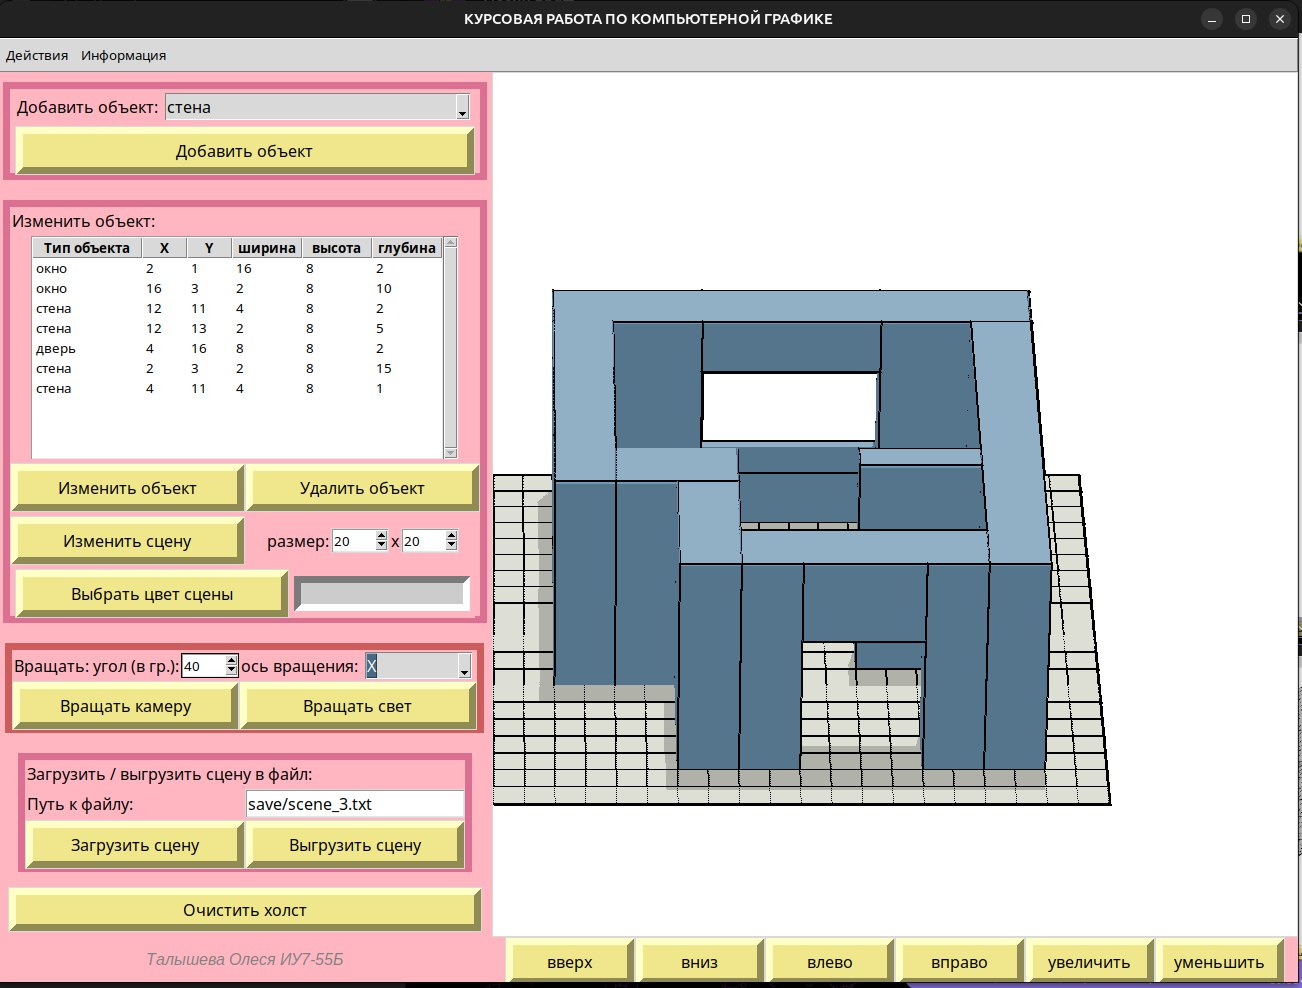
\includegraphics[width=1\textwidth]{img/example_light_10_0_0_camera_60_180_0.png}
    \caption{Интерфейс главного окна программного обеспечения.}
    \label{fig:main_interface}
\end{figure}

Программное обеспечение предлагает интуитивно понятный графический интерфейс для работы с 3D-сценами. Основной экран разделён на несколько функциональных областей, каждая из которых отвечает за выполнение конкретных задач (см. рисунок~\ref{fig:main_interface}).

В верхней части интерфейса находится блок для добавления объектов. Пользователь может выбрать тип объекта из выпадающего списка, например, "Окно" или "Стена" , после чего нажать кнопку "Добавить объект", чтобы добавить его в сцену (см. рисунок~\ref{fig:add_interface}). Все добавленные объекты отображаются в таблице в центральной части окна, где указаны их основные параметры: тип, координаты, размеры и глубина.

\begin{figure}[H]
    \centering
    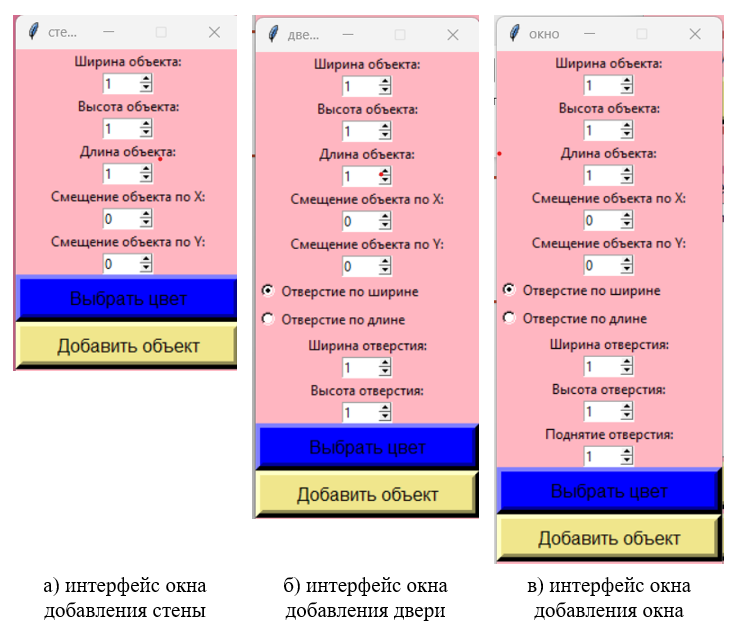
\includegraphics[width=1\textwidth]{img/add_interface.png}
    \caption{Интерфейс добавления объектов программы (а - стена, б - дверь, в - окно.}
    \label{fig:add_interface}
\end{figure}

Для изменения параметров уже существующих объектов предусмотрены кнопки "Изменить объект" и "Удалить объект". Это позволяет либо обновить свойства выбранного объекта, либо удалить его из сцены.

Кроме того, пользователь может настроить параметры сцены, задав её размер через соответствующие поля ввода и изменив цвет с помощью кнопки "Выбрать цвет сцены". Управление камерой также доступно — можно задать угол вращения вокруг выбранной оси (X, Y или Z).

Для сохранения или загрузки сцен предусмотрен функционал работы с файлами. Пользователь может указать путь к файлу и воспользоваться кнопками "Загрузить сцену" или "Выгрузить сцену", чтобы сохранить текущую сцену или восстановить её из файла. Также имеются кнопки для перемещения камеры вверх, вниз, влево или вправо, а также для изменения масштаба (увеличение или уменьшение).

При добавлении новых объектов, таких как окна или стены, открывается отдельное окно диалога. Например, при добавлении окна пользователь может указать его размеры, положение в сцене и параметры отверстия (ширина, высота и подъём). Есть возможность выбрать цвет объекта и, подтвердив настройки, добавить его в сцену. Для стен доступны аналогичные параметры, но без настройки отверстий.

Таким образом, интерфейс приложения предоставляет полный набор инструментов для создания и управления 3D-сценами, сохраняя удобство использования благодаря логично организованной структуре и понятным элементам управления.



\subsection{Выводы}

\hspace{1.25cm}
В данном разделе обоснован выбор языка программирования и инструментов, использованных для реализации проекта, проведён анализ структуры программы, включая назначение и взаимодействие её основных классов. Также было подробно рассмотрено устройство пользовательского интерфейса, включая функциональные возможности и элементы управления приложением.


\newpage